\documentclass{article}
\usepackage[preprint]{neurips_2026}

\usepackage[utf8]{inputenc}
\usepackage[T1]{fontenc}
\usepackage[hidelinks]{hyperref}
\usepackage{url}
\usepackage{booktabs}
\usepackage{amsfonts}
\usepackage{amsmath}
\usepackage{microtype}
\usepackage{xcolor}
\usepackage{graphicx}

% This is an ES 678 course paper, not a conference submission.
\makeatletter
\renewcommand{\@noticestring}{ES 678 Course Project}
\makeatother

\title{Finding Gujarat's Dumpsites from Free Satellite Data:\\ A Model Trained Elsewhere Finds the Sites but Not Only the Sites}

\author{%
  Amitesh Kumar \\
  Roll Number: 24210011 \\
  ES 678 \\
  Indian Institute of Technology Gandhinagar
}

\begin{document}
\maketitle

\begin{abstract}
Can a pixel classifier trained on Indian dumpsites outside Gujarat find Gujarat's dumpsites from free 10\,m satellite data, and when it is wrong, why? We hand-screened OpenStreetMap candidates and drew our own outlines to obtain 86 landfill places in 26 states, sampled 34,345 labelled pixels, and described each with 26 Sentinel-2, Landsat-thermal and SRTM features. Nine methods, from a published threshold rule to gradient boosting, were compared under region-held-out cross-validation, and the selected model was frozen under a Git tag before Gujarat was scored. It found 16 of 17 sealed Gujarat sites and 5 of 6 sites in a second, later list, but it also flagged 5.2\% of the scored land. A hand check of the 100 highest-ranked alarms found 5 dumpsites (3 previously unknown). The false alarms are not out-of-distribution: they look like training landfills, mainly through surface temperature. At realistic prevalence, pixel precision is below 2\%.
\end{abstract}

\section{Problem and Motivation}
Open dumpsites in India are poorly mapped, and published remote-sensing studies often report high scores on balanced test sets without checking what flagged places are \citep{bhajantri2026}; the one Sentinel-2 system whose detections were checked by people confirmed about half of its candidates, with two dates, a patch network, retraining on its own false alarms and human review \citep{kruse2023}. We ask: (Q1) does a model trained only outside Gujarat find Gujarat's known dumpsites; (Q2) how much does the validation design change the score; and (Q3) what precision should a user expect when dumpsites are rare? \textbf{Unit and target:} one row is one 10\,m pixel; the target is 1 if the pixel lies on visible active waste in March--May 2024, else 0. \textbf{Prediction time:} a prediction uses only imagery up to May 2024 and no Gujarat labels. The claim is limited to \emph{finding} pixels that resemble dumps; a flagged pixel is a candidate for a human check, not a confirmed site.

\section{Data and Preparation}
\textbf{Labels.} OpenStreetMap features tagged as landfill outside Gujarat were judged one by one by eye on 2024 imagery; 13 were kept and 93 dropped (60 of the drops are look-alikes: ash ponds, bare soil, quarries). We added 82 hand-drawn outlines of active sites; outlines within 500\,m are merged into one \emph{place}, giving 86 landfill places in 26 states. Sites under 1\,ha of visible waste were dropped (about one native Landsat thermal pixel). \textbf{Sampling.} Up to 50 points per landfill place (at least 15\,m inside the outline and 15\,m apart), up to 30 per look-alike place, random background across the source states, and 25,800 ``near-site'' background points in 15\,km boxes around training landfills, all at least 500\,m from any mapped site. After dropping 985 points with a missing value (snow or cloud), the table holds 34,345 points: 3,853 landfill (11.2\%), 24,989 near-site, 3,764 random and 1,739 look-alike. \textbf{Features (26).} Pre-monsoon (Mar--May 2024) Sentinel-2 medians of B2, B3, B4, B8, B11 with NDVI, NDBI and a bare-soil index; Landsat 8/9 land-surface temperature (LST) and $\mathrm{LST_{anom}}(x)=\mathrm{LST}(x)-\overline{\mathrm{LST}}_{\text{land},\,2\,\text{km}}(x)$, with permanent water \citep{pekel2016} excluded from the mean; SRTM elevation and slope \citep{farr2007}; a winter (Nov 2023--Feb 2024) composite of five bands and indices; 150\,m means and 50\,m standard deviations; and four differences (winter minus pre-monsoon, pixel minus neighbourhood). All are computed in Google Earth Engine \citep{gorelick2017}. \textbf{Leakage control.} The only learned preprocessing is the standardisation inside logistic regression, which is fit within each training fold by a scikit-learn pipeline; no Gujarat pixel, label or verdict is ever used in training. \textbf{Quality checks.} Every label is assigned to a state with geoBoundaries \citep{runfola2020}; points within 500\,m of any mapped site are never background; edge pixels are excluded by the 15\,m inset.

\section{Methods}
All models use scikit-learn defaults \citep{pedregosa2011}, class-balanced weights $w_i = n/(2n_{y_i})$ (with $n$ points and $n_{y}$ points of class $y$), and threshold 0.5 on the model score, with no tuning. \textbf{Baselines:} flag nothing (F1 = 0); the published rule NDBI $>0.028$, NDVI $<0.15$, LST $>37\,^\circ$C \citep{bhajantri2026}; and the same rule with cut-offs refit on training folds. \textbf{Learned models:} logistic regression on standardised features, a decision tree, bagged trees (200), random forest (500), AdaBoost (200 stumps) and gradient boosting (100 trees of depth 3, learning rate $\nu=0.1$). The selected model, gradient boosting, builds $F_M(\mathbf{x}) = F_0 + \nu\sum_{m=1}^{M} h_m(\mathbf{x})$, where each regression tree $h_m$ is fit to the negative gradient of the weighted log-loss $L=-\sum_i w_i[y_i\log p_i + (1-y_i)\log(1-p_i)]$ with $p_i=\sigma(F_{m-1}(\mathbf{x}_i))$ and $\sigma$ the logistic function; the model score is $p=\sigma(F_M(\mathbf{x}))$, flagged if $p\ge 0.5$. Trees suit the task because the features interact (a hot pixel is suspicious only if it is also bare) and their units differ. \textbf{Selection rule}, fixed before any result: the best mean F1 under region-held-out validation.

\section{Evaluation Design}
\textbf{Validation (selection only).} Only Maharashtra has 10 or more places, so the folds are India's six Zonal Council regions: each model is trained on five and tested on the sixth. Site-grouped and random-pixel five-fold splits are computed for contrast only. Precision, recall and F1 of the landfill class are reported as mean $\pm$ SD across folds. \textbf{Test.} The Gujarat list (17 outlined sites in 13 cities, $\ge$1\,ha) was sealed by commit before any model was run on Gujarat; the selected model was frozen under a Git tag before scoring, and the scoring script refuses to run on an untagged model. We scored a box 15\,km beyond each city's test sites (12,854\,km$^2$, about 6.6\% of Gujarat). A site is \emph{found} if at least half of its scored outline pixels are flagged. An \emph{alarm} is a 4-connected patch of flagged pixels of at least 1\,ha outside the sealed outlines, ranked by mean score. The 100 top alarms were judged blind on high-resolution imagery. A second list of 6 sites in 6 new cities was sealed later and scored once with the same frozen model.

\textbf{Disclosure.} This is the third frozen model scored on the first list. Version 1 (logistic regression, 12 features) found 16 of 17 sites, but none of its 50 top alarms that were checked was a dump (33 were blue roofs). Version 2 added the near-site background and ranked known sites below large bare patches. Version 3 added the winter and neighbourhood features. Its design responded to those failures, so the first list is no longer an unseen test; the new-cities list is. No Gujarat data entered any version's training.

\section{Results and Error Analysis}
\begin{table}[t]
\centering
\caption{Region-held-out validation (mean $\pm$ SD over six regions) and random-pixel F1, version~3 features. Gradient boosting is selected by the pre-set rule.}
\label{tab:val}
\small
\setlength{\tabcolsep}{4pt}
\begin{tabular}{lcccc}
\toprule
Method & Precision & Recall & F1 (region) & F1 (pixel) \\
\midrule
Published rule \citep{bhajantri2026} & 0.39 $\pm$ 0.08 & 0.55 $\pm$ 0.23 & 0.42 $\pm$ 0.14 & 0.45 \\
Recalibrated rule & 0.38 $\pm$ 0.18 & 0.58 $\pm$ 0.30 & 0.43 $\pm$ 0.22 & 0.50 \\
Logistic regression & 0.59 $\pm$ 0.12 & 0.90 $\pm$ 0.10 & 0.70 $\pm$ 0.07 & 0.72 \\
Random forest & 0.85 $\pm$ 0.08 & 0.67 $\pm$ 0.17 & 0.74 $\pm$ 0.11 & 0.91 \\
AdaBoost & 0.60 $\pm$ 0.07 & 0.88 $\pm$ 0.10 & 0.71 $\pm$ 0.04 & 0.73 \\
\textbf{Gradient boosting} & 0.69 $\pm$ 0.09 & 0.86 $\pm$ 0.10 & \textbf{0.76 $\pm$ 0.04} & 0.81 \\
\bottomrule
\end{tabular}
\end{table}

\textbf{Validation.} Every learned model beats both threshold rules by about 0.3 F1 (Table~\ref{tab:val}; tree and bagging, omitted, score 0.63 and 0.68). Gradient boosting has the best region F1, 0.762, though within one SD of the random forest. \textbf{Gujarat (Q1).} The frozen model found 16 of 17 sealed sites; Rajkot was missed with 48.6\% of its outline flagged, just under the rule. In the new cities it found 5 of 6 (Porbandar missed), so 21 of 23 overall. But it flagged 5.2\% of the scored land, in 7,801 alarm patches (4.0\% of 5,244\,km$^2$ in the new cities). Ranked with the sealed sites left in, patches of known sites hold 5 of the top 50 and 8 of the top 100. A landfill on neither list, at Surendranagar, ranks 4th.

\textbf{Error analysis.} Of the 100 top alarms, 5 were dumpsites (3 previously unknown), 94 look-alikes and 1 unsure: a precision of 5.1\% among decided alarms (95\% Clopper--Pearson interval 1.7--11.4\%). The look-alikes were bare or excavated soil (46), fields or grass (19), buildings (16), industrial yards (5) and other (8). The same confusion is visible in validation: the model flags 16\% of bare-soil, 20\% of quarry and 12\% of ash-pond points, against 3.2\% of random background.

\section{Graduate Depth Analysis}
\begin{figure}[t]
\centering
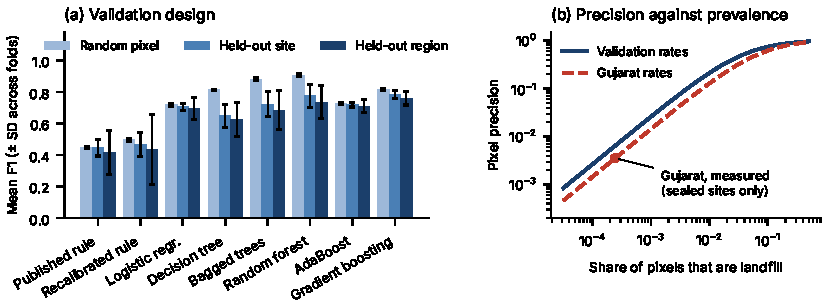
\includegraphics[width=\linewidth]{figures/fig_main.pdf}
\caption{(a) Mean F1 under three validation designs; trees gain most from random-pixel splits. (b) Expected pixel precision $\pi(\rho)$ against landfill prevalence $\rho$, from validation and Gujarat rates; the dot is the measured Gujarat value against the sealed list.}
\label{fig:main}
\end{figure}

\textbf{Split ablation (Q2).} Random-pixel splits put pixels from the same site on both sides, so they reward memorising sites. Figure~\ref{fig:main}a shows the effect is model-dependent: the random forest falls from 0.907 (random pixel) to 0.775 (held-out site) to 0.736 (held-out region), the decision tree from 0.815 to 0.625, but gradient boosting only from 0.815 to 0.762 and logistic regression from 0.719 to 0.697. Under random-pixel validation the forest would have been selected. Gujarat adds a fourth rung: at pixel level, 75.4\% of outline pixels and 5.17\% of all other pixels are flagged. At the validation class mix (11.2\% landfill) this would give F1 0.70, close to validation. So the score falls only modestly with distance; the failure lies elsewhere.

\textbf{Precision against prevalence (Q3).} With recall $r$ and false-alarm rate $f$, precision at prevalence $\rho$ is $\pi(\rho) = r\rho/(r\rho + f(1-\rho))$. Validation rates ($r=0.864$, $f=0.032$ on random background) give $\pi=96\%$ at $\rho=0.5$ but 21\% at $\rho=1\%$ and 2.6\% at $\rho=0.1\%$; Gujarat rates give 13\% and 1.4\% (Fig.~\ref{fig:main}b). In the scored boxes, sealed outlines are 0.024\% of pixels, and the measured pixel precision against the sealed list is 0.35\%. That is a lower bound, since unlisted dumps count as false alarms, but it matches the curve. Balanced-test scores therefore say little about usefulness: the false-alarm rate, not recall, decides precision.

\textbf{Failure audit: are the alarms out of distribution?} For each hand-checked alarm centre we found its 15 nearest training points in standardised feature space. None of the 94 look-alike alarms lies beyond the 99th percentile of training-point distances (median percentile 45), and 80 of 94 have a landfill as the nearest training point. Mean SHAP values \citep{lundberg2017} show what pushes them over the threshold: thermal features add $+2.43$ log-odds for look-alike alarms against $+1.83$ for the sealed sites, while spectral, winter and neighbourhood features add more for real dumps ($+0.86$, $+0.54$, $+0.40$) than for look-alikes ($+0.29$, $+0.19$, $+0.11$). $\mathrm{LST_{anom}}$ alone separates landfill from random background with AUC 0.94 and carries a third of the model's SHAP mass. The false alarms are therefore not a distribution-shift failure that more Gujarat-like data would fix. They are hot, bare places that share the dumps' main signature at 10--100\,m. Version 1 failed differently: its alarms were out of distribution (20--26\% beyond the 99th percentile; blue roofs extrapolated by a linear model). Version 3 corrected that, but not the thermal confusion.

\section{Limitations and Conclusion}
The most important limitation is the test design. The first list has now been seen by three versions, and the second has only 6 sites; a stronger claim needs a larger list sealed in advance and a random sample of alarms, not only the top 100, checked on the ground. Recall is measured on known sites only, which favours large, well-known dumps. Only 6.6\% of Gujarat was scored, and unscored land is not ``clean''. Associations between temperature and waste are predictive, not causal. \textbf{Conclusion.} A model trained outside Gujarat does find Gujarat's dumpsites (21 of 23), and region-held-out validation predicts its pixel-level behaviour well. But it cannot be used as a shortlist on its own. At realistic prevalence it yields 1--5\% precision because thermal anomaly, its strongest cue, is shared by bare and industrial land. It is useful as a first filter for a human check, which here found three unlisted sites in 100 alarms; closing the gap to the roughly 50\% confirmation rate of \citet{kruse2023} likely needs whole-patch context rather than more pixel features.

\section{Reproducibility and AI-Use Disclosure}
Code, labels, sample points, feature tables, frozen models (tags \texttt{freeze-v1}--\texttt{v3}), per-pixel Gujarat scores and the hand-check sheet are at \url{https://github.com/wre9-tesh/ML_Landfill_Detection}; the README gives the run order. Steps other than the Earth Engine fetches run from the repository without an account; the Gujarat rasters are rebuilt from public data with a free Earth Engine account. No credentials are stored. \textbf{AI use.} Claude (Anthropic), through Claude Code, wrote the Python scripts to the author's specification, ran training and diagnostics, searched for related work and drafted documentation and this paper's text. The author chose the question, screened every candidate, drew every outline, compiled the test lists, ran the Earth Engine fetches and Gujarat scoring, judged all 100 alarms, and checked every number against the result files. No label or verdict was produced by AI.

{\small
\bibliographystyle{plainnat}
\bibliography{refs}
}

\end{document}
